Eine Kiste liegt auf einer schiefen Ebene mit Neigungswinkel \wiO. Sie ist über ein leichtes Seil mit einer zweiten Kiste der Masse $m_2 = \mZwO$ verbunden, die in der Luft hängt.

\begin{center}
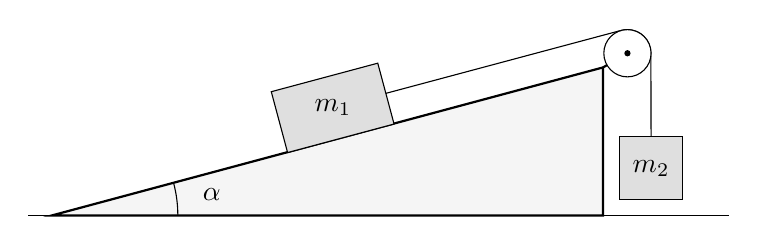
\begin{tikzpicture}[>=stealth]
 \draw[thick, fill=gray!8] (0,0) -- (7.00,0) -- (7.00,1.88) -- cycle;
 \draw (-0.3,0) -- (8.60,0);
 \draw (1.6,0) arc (0:15:1.6);
 \node at (2.03,0.27) {$\alpha$};
 \begin{scope}[shift={(3.67,0.98)}, rotate=15]
  \draw[fill=gray!25] (-0.7,0) rectangle (0.7,0.8);
 \end{scope}
 \node at (3.57,1.37) {$m_1$};
 \draw[thick] (7.00,1.88) -- (7.31,2.06);
 \draw (4.24,1.55) -- (7.23,2.35) arc (105:0:0.3) -- (7.61,1.0);
 \draw[fill=white] (7.31,2.06) circle (0.3);
 \fill (7.31,2.06) circle (0.04);
 \draw[fill=gray!25] (7.21,0.2) rectangle (8.01,1.0);
 \node at (7.61,0.6) {$m_2$};
\end{tikzpicture}
\end{center}

\begin{abcliste}
\abc Wie schwer muss die erste Kiste sein, damit Gleichgewicht herrscht?
\abc Berechnen Sie die Beschleunigung (inkl. Richtung) der beiden Kisten, wenn die erste Kiste \mEiO\ schwer ist. Die Reibung kann vernachlässigt werden.
\abc Wie gross ist in der Situation von b) die Seilkraft, d.h. die Kraft, mit welcher das Seil an $m_1$ bzw. $m_2$ zieht?
\end{abcliste}
